\chapter{Rotation Matrices} \labchap{rotation_matrix}
A rotation matrix is a mathematic model for translating one body's inertial reference frame to another, e.g. local frame to a global frame.
These are used for Eulerian transformations of vectors (i.e. using roll, pitch, and yaw).
To begin deriving these matrices, let's start with a two dimensional rotation matrix:

\begin{equation*}
    R(\theta) = \left[
        \begin{matrix}
            \cos\theta & -\sin\theta \\
            \sin\theta & cos\theta
        \end{matrix}\right]
\end{equation*}

If we rotate a vector, $\vec{v} = \langle x, y \rangle$ with a magnitude, $r$ by $\theta$ degrees about the Z-axis (as shown in Figure \ref{fig:2d_rot}), it will arrive at a new coordinate $\langle x^{\prime}, y^{\prime}\rangle$. 
We can express $\vec{v}$ in polar form as:

\begin{align}
    x &= r\cos\phi \\
    y &= r\sin\phi
\end{align}

Similarly, the rotated vector, $\vec{v}^{\prime}$ in polar form is expressed as:

\begin{align*}
    x^{\prime} &= r\cos(\phi+\theta) \\
    y^{\prime} &= r\sin(\phi+\theta)
\end{align*}

\begin{figure}[h!]
    \caption{2 dimensional rotation of a vector, $A$, to a new set of coordinates, $A'$.}
    \labfig{2d_rot}
    \centering
    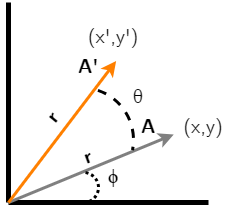
\includegraphics[height=2.5in]{appendices/rotation_matrix/2d_rotation_plot.png}
\end{figure}

Expanding and using trigonometric identities:

\begin{align*}
    x^{\prime} &= r(\cos\phi\cos\theta + \sin\phi\sin\theta) \\
               &= r\cos\phi\cos\theta + r\sin\phi\sin\theta \\
               &= x\cos\theta + y\sin\theta \\
    y^{\prime} &= r(\sin\phi\sin\theta + \cos\phi\sin\theta) \\
               &= r\sin\phi\cos\theta + r\cos\phi\sin\theta \\
               &= y\cos\theta + x\sin\theta
\end{align*}

We can then express the resultant equations in the form of a $2 \times 2$ rotation matrix, $R$, yielding:

\begin{equation*}
    \left[
        \begin{matrix}
            x^{\prime} \\ 
            y^{\prime}
        \end{matrix}
    \right]
    =
    \left[
        \begin{matrix}
            \cos\theta & -\sin\theta \\
            \sin\theta & \cos\theta
        \end{matrix}
    \right]
    \left[
        \begin{matrix}
            x \\
            y
        \end{matrix}
    \right]
    = R(\theta)
    \left[
        \begin{matrix}
            x \\
            y
        \end{matrix}
    \right]
\end{equation*}

\paragraph*{Example} If we have a vessel moving in the a direction at some velocity and it encounters a current, $\vec{v}$ coming in from the starboard quarter, what is the current's influence on the vessel?

\begin{figure}[h!]
    \caption{A vessel encounters a current (orange), $\pmb{v}$, from the forward starboard quarter.}
    \labfig{boat_current}
    \centering
    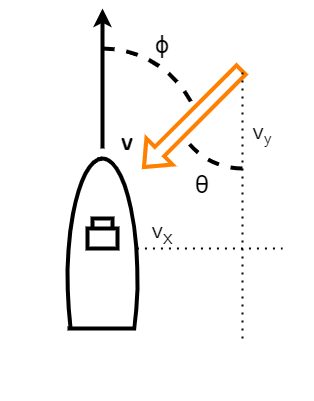
\includegraphics[height=2.5in]{appendices/rotation_matrix/boat_current.png}
\end{figure}

First, we can use the parallel axis theorem to determine that the current is impinging on the vessel at an angle, $\theta$, relative to its longitudinal (y) axis.
We can consider the current vector to be in the global frame and to find its influence on the vessel, we must rotate it to the vessel's local frame and get the resultant vector, $[v_x, v_y]$.
Using a rotation matrix, we can determine that:

\begin{equation*}
    \left[
        \begin{matrix}
            v_x^{\prime} \\
            v_y^{\prime}
        \end{matrix}
    \right] = 
    R(\theta) \left[
        \begin{matrix}
            v_E \\
            v_N
        \end{matrix}
    \right]
\end{equation*}

\section{Three Dimensional Rotation Matrix} \labsec{3d_rot_mat}
In three dimensional space, rotation can be performed about the X-, Y-, or Z-axis. A basic rotation that occurs around a single axis is defined as an "elementary rotation" and given by the following rotation matrices:

\begin{align*}
    R_x(\phi) &= \left[
        \begin{matrix}
            1 & 0 & 0 \\
            0 & \cos\phi & -\sin\phi \\
            0 & \sin\phi & \cos\phi
        \end{matrix}
    \right] \\
    R_y(\theta) &= \left[
        \begin{matrix}
            \cos\theta & 0 & \sin\theta \\
            0 & 1 & 0 \\
            -\sin\theta & 0 & \cos\theta
        \end{matrix}
    \right] \\
    R_z(\psi) &= \left[
        \begin{matrix}
            \cos\psi & -\sin\psi & 0 \\
            \sin\psi & \cos\psi & 0 \\
            0 & 0 & 1
        \end{matrix}
    \right]
\end{align*}

To rotate a three dimensional vector from one frame to another, we must select the order of the axes to be rotated about, then multiply the rotation matrices and vector together.
\paragraph*{Example} What are the components of gravitational acceleration, $a_G$ that affect an airplane in flight at some arbitrary roll ($\phi$), pitch ($\theta$), and yaw ($\psi$)?

\begin{figure}[h!]
    \caption{A plane rotated at some arbitrary roll (red), $\phi$, pitch (blue), $\theta$, and yaw (green), $\psi$, experiences gravitational acceleration in all three axes.}
    \labfig{airplane_rotation}
    \centering
    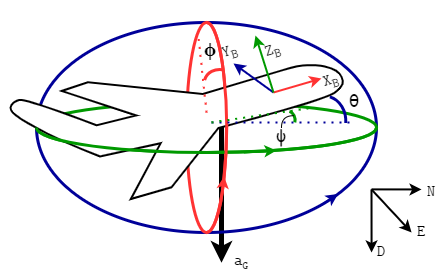
\includegraphics[height=2.5in]{appendices/rotation_matrix/airplane_rotation.png}
\end{figure}

First, we define the gravitational acceleration vector as existing in the global North-East-Down (NED) reference frame, $a_G = \langle a_N, a_E, a_D \rangle = \langle 0, 0, 1 \rangle$.
We will also assume that all of the rotations of the plane are relative to the same NED frame.
We can then perform a yaw-pitch-roll rotation of $a_G$ to get the gravitational acceleration in terms of the plane's coordinate frame, ${}^G_B a$:

\begin{align*}
    {}^G_B a &= R_z(\psi) R_y(\theta) R_x(\phi) a_G \\
    &= 
    \left[
        \begin{matrix}
            \cos\psi & -\sin\psi & 0 \\
            \sin\psi & \cos\psi & 0 \\
            0 & 0 & 1
        \end{matrix}
    \right]
    \left[
        \begin{matrix}
            \cos\theta & 0 & \sin\theta \\
            0 & 1 & 0 \\
            -\sin\theta & 0 & \cos\theta
        \end{matrix}
    \right]
    \left[
        \begin{matrix}
            1 & 0 & 0 \\
            0 & \cos\phi & -\sin\phi \\
            0 & \sin\phi & \cos\phi 
        \end{matrix}
    \right] 
    \left[
        \begin{matrix}
            0 \\
            0 \\
            1
        \end{matrix}
    \right]\\
    {}^G_B a &= 
    \left[
        \begin{matrix}
            \cos\psi\cos\theta & \cos\psi\sin\theta\sin\phi-\sin\psi\cos\theta & \cos\psi\sin\theta\cos\phi+\sin\psi\sin\phi \\
            \sin\psi\cos\theta & \sin\psi\sin\theta\sin\phi+\cos\psi\cos\phi & \sin\psi\sin\theta\cos\phi-\cos\psi\sin\phi \\
            -\sin\theta & \cos\theta\sin\phi & \cos\theta\cos\phi
        \end{matrix}
    \right]
    \left[
        \begin{matrix}
            0 \\
            0 \\
            1
        \end{matrix}
    \right]
\end{align*}